\documentclass[final,supplement,onefignum,onetabnum]{siamart171218}

% This is information that is shared between the main document and any
% supplement. If no supplement is required, then this information can
% be included directly in the main document.


% Packages and macros go here
\usepackage{lipsum}
\usepackage{amsfonts}
\usepackage{graphicx}
\usepackage{epstopdf}
\usepackage{algorithmic}
\usepackage{tikz}
\usepackage{subcaption} 
\usepackage{pc_math}
\usepackage{amssymb}
\usepackage{bbm}
% \usepackage[color=gray!60]{todonotes}
\usepackage[disable, color=gray!60]{todonotes}
% \usepackage{caption}
% \usepackage{hyperref}
\graphicspath{{fig/}}

\tikzstyle{major}=[circle, fill=blue!50, minimum size=10pt, line width=0mm, inner sep=0pt, draw=black]
\tikzstyle{minor} = [major, fill=orange!80, draw=black]
\tikzstyle{focus} = [minor, line width=.2mm, inner sep=1pt, draw=black]
\tikzstyle{edge} = [draw,line width=.3mm, -, gray!120]
\tikzstyle{gone} = [edge,  densely dotted]
\tikzstyle{arrow} = [draw,line width=.2mm, ->, gray!120]


\tikzstyle{weight} = [font=\small]

\ifpdf
  \DeclareGraphicsExtensions{.eps,.pdf,.png,.jpg}
\else
  \DeclareGraphicsExtensions{.eps}
\fi

% Add a serial/Oxford comma by default.
\newcommand{\creflastconjunction}{, and~}

% Used for creating new theorem and remark environments
\newsiamremark{remark}{Remark}
\newsiamremark{hypothesis}{Hypothesis}
\crefname{hypothesis}{Hypothesis}{Hypotheses}
\newsiamthm{claim}{Claim}

% Sets running headers as well as PDF title and authors
\headers{Adaptive Voter Models}{P. Chodrow, P. J. Mucha}

% Title. If the supplement option is on, then "Supplementary Material"
% is automatically inserted before the title.
\title{Symmetry-Breaking in Adaptive Voter Models\thanks{Submitted to the editors \today.
\funding{This work was funded by the NSF (1122374).}}}

% Authors: full names plus addresses.
\author{Philip S. Chodrow\thanks{Operations Research Center, Massachusetts Institute of Technology, Cambridge, MA, 02139 and Laboratory for Information and Decision Systems, Massachusetts Institute of Technology, Cambridge, MA, 02139
  (\email{pchodrow@mit.edu}, \url{http://www.philchodrow.github.io}).}
\and Peter J. Mucha\thanks{Carolina Center for Interdisciplinary Applied Mathematics, Department of Mathematics, University of North Carolina, Chapel Hill, NC 27599-3250, and Department of Applied Physical Sciences, University of North Carolina, Chapel Hill, NC 27599-3050. 
  (\url{http://mucha.web.unc.edu/}).}}

\usepackage{amsopn}
%%% Local Variables: 
%%% mode:latex
%%% TeX-master: "ex_article"
%%% End: 


\externaldocument{main}

% Optional PDF information
\ifpdf
\hypersetup{
  pdftitle={Adaptive Voter Models},
  pdfauthor={P. Chodrow and P. Mucha}
}
\fi

\begin{document}

\maketitle

\section{Distribution of Opinion Densities}
  In this section, we show that $\mathbf{q}_1$ converges in measure to a uniform random variable on the space of possible opinion densities. 
  \begin{lemma} \label{lm:uniform}

    Let $\mu_{\lambda,n}$ be the equilibrium measure of $\mathbf{q}_1$. 
    Then, 
    \begin{align}
       \lim_{\lambda \rightarrow 0}\mu_{\lambda, n}(q|q\notin \{0,1\}) = \frac{1}{n}\;.
    \end{align} 
  \end{lemma}
  \begin{proof}
  \todo{touch up this proof}

    To see this, we note that $N_1(t)$ is a birth-death process on the states $[N]$, with transition probabilities
    \begin{align*}
      b_n &\triangleq \prob(N_1(t+1) = n+1 | N_1(t) = n) = \lambda \frac{N - n}{N} + (1-\lambda)\frac{1}{2}\\ 
      d_n &\triangleq \prob(N_1(t+1) = n-1 | N_1(t) = n) = \lambda \frac{n}{N} + (1-\lambda)\frac{1}{2}\;.
    \end{align*}
    The equilibrium distribution $\pi$ of this chain satisfies 
    \begin{align*}
      \pi_n &= \pi_0\prod_{i = 1}^n \frac{b_{i - 1}}{d_{i}}  \\ 
          &= \pi_0\prod_{i = 1}^n \frac{2\lambda (N-i+1) + N(1-\lambda)}{2\lambda i + N(1-\lambda)}\;. 
    \end{align*}
    The product converges to $1$ as $\lambda \rightarrow 0$. 
    This implies that $\pi_n \rightarrow \pi_0$ for all $n$; that is, $\pi$ converges to the uniform distribution on $[N]$. 
    The proportion $U$ therefore converges to a discrete uniform random variable on $\left\{0,\frac{1}{N}, \ldots,\frac{N-1}{N}, 1\right\}$. 
    Informally, for small $\lambda$, $\mathbf{u}$ is nearly uniform on $[0,1]$. 
    That is, while the AVM behavior is indeed symmetric about the point $u_1 = \frac{1}{2}$, it will spend much of its time far away from this point unless $\lambda$ is large. 
  \end{proof}

\section{Symmetry Breaking in Simulation Data} \label{sec:simulation_symmetry}
    The asymmetric behavior of forward and backward votes may be observed in simulation data. 
    \Cref{fig:symmetry_breaking} shows the distribution of the change in $M_{01} = \rho m$ due to voting events for varying values of $\rho$. 
    At small values of $\rho$ for which the distinction between forward and backward votes is sharp, the distribution is weakly bimodal. 
    The peak corresponding to forward votes is positive, while the peak corresponding to backward votes is negative. 
    A mean-field estimate for $\Delta M_{01}$ due to forward voting events is $\E[\Delta M^{\rightarrow}_{01}] \approx c(1-2\rho) - 1$, with the first term accounting for edges attached to the node that votes and the second term accounting for the active edge along which the vote takes place. 
    This quantity is shown as the red vertical line in \cref{fig:symmetry_breaking}, and may be compared to the overall mean shown in black.  
    The rewiring and voting processes \cref{fig:breaking_illustration} tend to reduce the impact of backward votes, implying that the overall mean is positive. 
    As $\rho$ increases, the forward-backward asymmetry fades away, eventually yielding a symmetric, approximately Gaussian distribution centered near $0$.  

    \begin{figure}
      \centering
        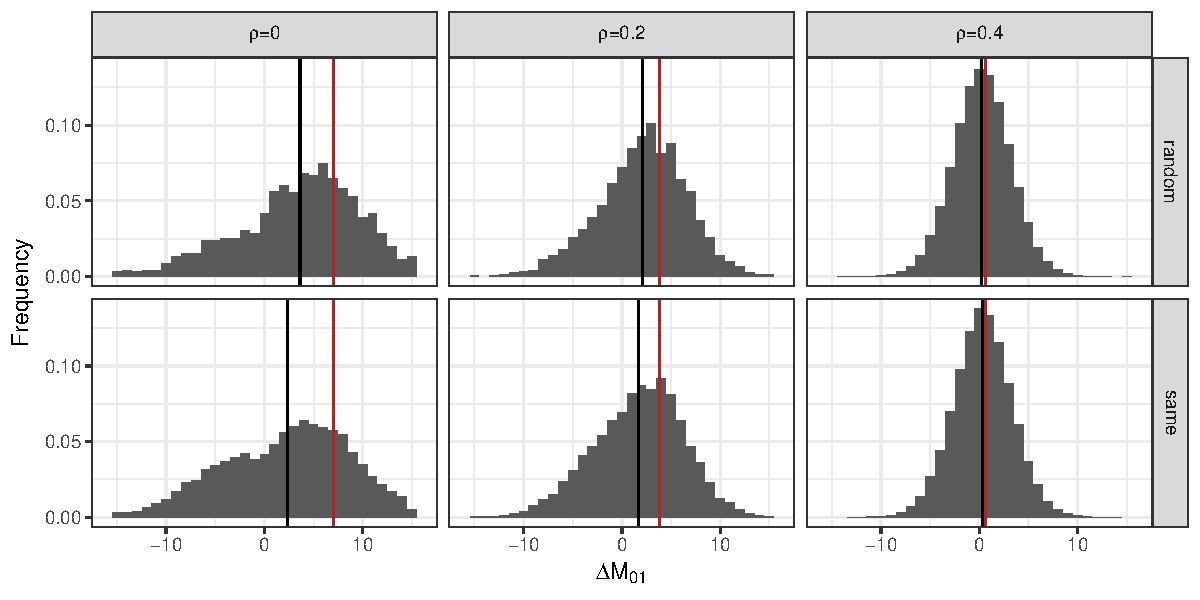
\includegraphics[width=1\textwidth]{symmetry_breaking}
      \caption{
      Observed symmetry-breaking in the adaptive voter model. 
      Observed distribution of the change in active link count $M_{01}$ due to voting events.  
      The data shown is from a model with $c = 8$, $n = 10^4$, and $\lambda = 2^{-8}$, with varying $\alpha$. 
      The black vertical gives the mean of the distribution, while the red vertical gives the mean-field estimate $\E[\Delta M^{\rightarrow}_{01}] \approx c(1-2\rho) - 1$ for the mean change due to forward voting events only. 
      } \label{fig:symmetry_breaking}
    \end{figure}


\section{Computation of $\hat{v}$} \label{sec:calcs}

  We now proceed to compute the required components of $\hat{v}(\mathbf{q}, \mathbf{x}|I, J_0, K_0)$ defined in the main text. 
  We begin with $K$, the active edge count at the time that $u$ votes. 
  It is distributed as 
  \begin{align*}
    p_{K|I, K_0}(k|i, k_0) = 
    \begin{cases}
      (1-\beta_i)\beta_i^{k_0 - k} &\quad 1\leq k \leq k_0\\ 
      \beta_i^{k_0} &\quad k = 0,
    \end{cases}
  \end{align*}
  where $\beta_i$ is the probability that an event is not a vote by $u$, given that it removes a discordant edge from $u$. 
  It is given analytically by 
  \begin{align*}
    \beta_i \triangleq 
    \begin{cases}
      \frac{1+\alpha q_i}{2-\alpha(1-q_i)} &\quad \text{rewire to same}\\ 
      \frac{1+\alpha}{2} &\quad \text{rewire to random.}
    \end{cases}
  \end{align*}
  We similarly define the coefficients 
 \begin{align*}
    \eta_i \triangleq 
    \begin{cases}
      \frac{1-\alpha(1-q_i)}{1+\alpha q_i}  \\ 
      \frac{1-\alpha}{1+\alpha} 
    \end{cases} \quad 
    \rho_i \triangleq 
    \begin{cases}
      \frac{1-\alpha}{1+\alpha q_i}  \\ 
      \frac{1-\alpha}{1+\alpha}   
    \end{cases} \quad 
    \sigma_i \triangleq 
    \begin{cases}
      \frac{2(1-\alpha)}{2-\alpha} &\quad \text{rewire to random} \\ 
      0   &\quad \text{rewire to same.}
    \end{cases}
  \end{align*}
  The coefficient $\eta$ gives the probability that an event that removes a discordant edge from $u$, other than a vote by $v$, produces a concordant edge either through rewiring or through a vote by a neighbor of $v$. The coefficient $\rho$ gives the probability that such an event is in fact a vote by a neighbor of $v$. The coefficient $\sigma$ gives the probability that an edge which is rewired but not resolved is ultimately resolved via a vote. 

  We may now compute the various terms in \Cref{eq:component_approx}. First, 
  \begin{align*}
    \prob(\1_u = 1) &= \prob(K \geq 1) \\ 
             &= 1-\beta_i^{K_0}.
  \end{align*}
  Averaging over $K_0$ yields
  \begin{align*}
    \E[\1_u|i] = \sum_{k_0}p_{K_0}(k_0)(1-\beta_i^{k_0}) = 1 - \phi_{K_0}(\beta_i)\;.
  \end{align*}
  The expected number of discordant edges at time of voting, can be computed as 
  \begin{align*}
    \E[\1_uK|i] &= \E_{K_0}\E[\1_uK|i, K_0] \\ 
                &= \E_{K_0}\left[K_0 - \frac{\beta_i(1-\beta_i^{K_0})}{1-\beta_i}|i\right] \\ 
                &= \E[K_0|i] - \frac{\beta_i}{1-\beta_i}(1-\phi_{K_0}(\beta_i))\;.
  \end{align*}
  Node $u$ gains concordant edges via rewiring and voting at rate $\eta_i$. The expected number of concordant edges at the time of that $u$ votes is therefore 
  \begin{align*}
    \E[\1_uJ|i] &= \E_{K_0}\left[\E[J_0|i, K_0] + \eta_i \left(\E[K_0|i] - \E[1_uK|i, K_0]\right)\right] \\
                &= \E[K_0|i] + \eta_i \left(\E[K_0|i] - \E[\1_uK|i]\right)\;.
  \end{align*}
  Next, the expected number $\E[R|i]$ of votes by neighbors of $u$ can be calculated simply by noting that a voting event along edge $(u,v)$ has equal probability to change $\mathcal{L}_u$ as $\mathcal{L}_v$. 
  As a result, the expected number of votes by neighbors is the same as the expected number of votes by $u$ itself, which is simply $\E[\1_u|i]$. We thus obtain 
  \begin{align*}
    \E[R|i] = \E[\1_u|i] = 1 - \phi_{K_0}(\beta_i)\;. 
  \end{align*}
  Finally, we calculate the expected number $W$ of votes by nodes not attached to $v$. 
  First, the voting edge must be no longer attached to $u$. 
  The expected number of such edges is $\E[K_0 + J_0 - \1_u(K - J)|i]$. 
  The probability that such an edge was removed by $u$ by a rewiring event that did not resolve the edge is $\sigma_i$. 
  We thus have 
  \begin{align*}
    \E[W|i] = \sigma_i\E[K_0 + J_0 - \1_u(K - J)|i]\;.
  \end{align*}

\section{Mean-Field Approximation for $\alpha = 0$} \label{sec:SI_alpha_0}
  In this section, we derive \Cref{eq:alpha_0} of the main text, which gives a mean-field approximation for the arch in the case $\alpha = 0$. 
  In this case, active edges enter and exit the system only via voting events. 
  The mean-field approximation for the impact of a voting event is $g(\C) = \frac{1}{2}\left(h_0(\C) + h_1(\C)\right)$, where $h_i(\C)$ is defined in the main text. 
  The equilibrium condition is $g(\C) = 0$. 
	Since $\C$ lives in a 2-dimensional subspace of $\R^4$, it suffices to solve the system
	\begin{align*}
		0 &= g_{00}(\C) = 1 + c_{10} - c_{00} \\ 
		0 &= g_{11}(\C) = 1 + c_{01} - c_{11} 
	\end{align*}
	for $\C$ and subsequently for $\x$.  
  We recall that $c_{ij} = c\frac{x_{ij}}{q_i}$ and that $2x_{01} = 1 - x_{00} - x_{11}$. 
  Substituting, we obtain 
  \begin{align*}
    0 &= 1 +c \left(\frac{1 - x_{00} - x_{11}}{2q_1}  - \frac{x_{00}}{q_0}\right) \\ 
    0 &= 1 +c \left(\frac{1 - x_{00} - x_{11}}{2q_0}  - \frac{x_{11}}{q_1}\right) 
  \end{align*}
  or 
  \begin{align*}
    \frac{2q_0q_1}{c}\mathbf{e} + \q = \left[\begin{matrix} 1 + q_1 & q_0 \\ q_1 & 1 + q_0 \end{matrix}\right]\left(\begin{matrix}x_{00} \\ x_{11}\end{matrix}\right)\;.
  \end{align*}
  The unique solution is 
  \begin{align*}
    \left(\begin{matrix}x_{00} \\ x_{11}\end{matrix}\right) = \frac{q_0 q_1}{c} \mathbf{e} + \frac{1}{2}\left(\begin{matrix} q_0(1 + q_0 - q_1) \\ q_1(1 + q_1 - q_0) \end{matrix}\right)\;.
  \end{align*}
  We may then compute the arch: 
  \begin{align*}
    \rho &= 2x_{01} \\ 
         &= 1 - x_{00} - x_{11} \\ 
         &= 2q_0 q_1 \frac{c-1}{c}\;,
  \end{align*}
  as was to be shown. 
	



	
	
	




% \bibliographystyle{siamplain}
% \bibliography{/Users/phil/bibs/library.bib}{}


\end{document}
